\newpage\thispagestyle{hl}
\hlbanner{The whole book}{}{At a glance}
\hlsection{What the book is}
\begin{hlquote}This book describes how a reduced-order modelling package, \rom{}, is built on top of a finite element package, \fea{}, for the analysis of structures, and checks, one claim at a time, that the two packages do what is said of them.\end{hlquote}
It is written for readers who already know the finite element method and the idea of model reduction, and who want to see how the two meet in working code. Every listing was run, and every number in the text is generated by a script and enters the book as a macro.
\hlsection{The two packages and how they meet}
\begin{center}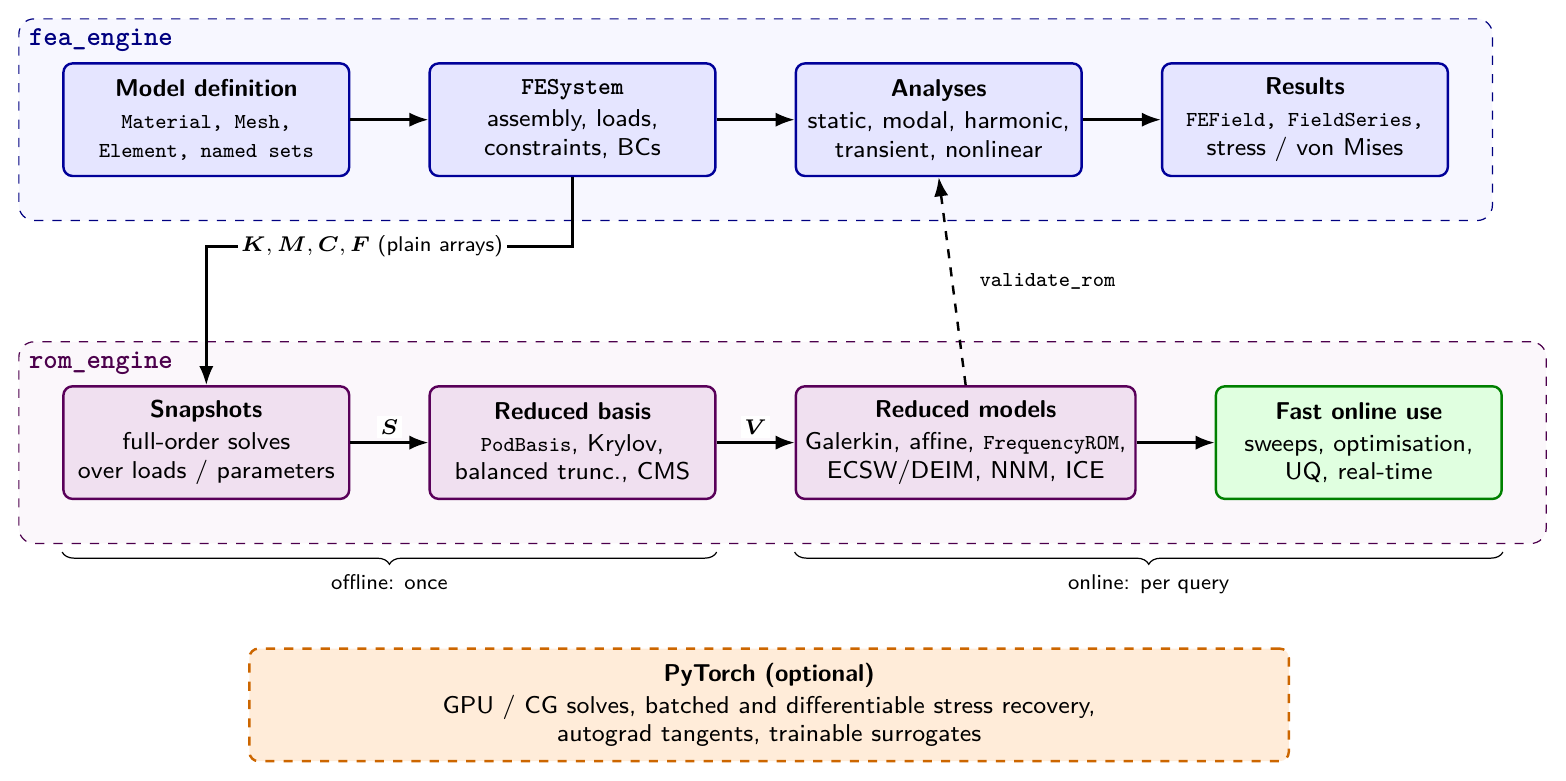
\includegraphics[width=\linewidth]{figures/architecture.png}\end{center}
{\small\color{hlgrey}\textbf{Figure.} \fea{} produces the matrices and the full-order solutions; \rom{} works on plain arrays, never imports \fea{}, and returns reduced models for fast online use.}
\hlsection{Four parts, fourteen chapters}
{\small\begin{tabularx}{\linewidth}{@{}p{0.27\linewidth}>{\raggedright\arraybackslash}p{0.1\linewidth}X@{}}
\textsf{\textbf{\color{hlnavy}Architecture}} & Ch.\ 1--2 & the design of the engine, and meshes that are checked rather than assumed \\[3pt]
\textsf{\textbf{\color{hlnavy}Full-order physics}} & Ch.\ 3--7 & elements and locking, dynamics, nonlinearity, batched assembly, exact contact \\[3pt]
\textsf{\textbf{\color{hlnavy}Reduced-order modelling}} & Ch.\ 8--13 & POD--Galerkin, balanced truncation, Krylov and SOAR, frequency-domain and greedy, substructuring, non-intrusive and nonlinear, hyper-reduction and contact \\[3pt]
\textsf{\textbf{\color{hlnavy}Verification}} & Ch.\ 14 & what ``verified'' means, nine reproduction studies, an integrated pipeline \\
\end{tabularx}}
{\small Four appendices follow: differentiable assembly, conventions and tolerances, a glossary, and a map from chapters to the package tests that cover them.}

\newpage\thispagestyle{hl}
\hlbanner{The whole book}{}{How it is built}
\hlsection{Six levels of evidence}
\hlfig{\hltikz{ch14_pyramid}}{Each number in the book sits on one of six levels, from a unit test to an integrated run. The references are never the code under test.}
\hlsection{Every chapter has the same layout}
An opening box and a concrete problem; the mathematical structure; the implementation in the packages, with pseudocode, cost and failure modes; a Verification section; a box of limits; a summary; exercises of three kinds (derivation, implementation, interpretation). Short boxes inside the text define terms where they are first needed.
\hlsection{Nine published studies, rebuilt from the packages}
{\small\begin{tabularx}{\linewidth}{@{}>{\raggedright\arraybackslash}p{0.5\linewidth}X@{}}
Multi-fidelity surrogate ROM (He, 2023) & reproduced; one reference fails at large amplitude \\
Hybrid modal ROM (Yang, 2019) & reproduced on a panel; open defect on a plate \\
Implicit condensation and expansion (Hollkamp, 2008) & statics reproduced; dynamics not \\
Loewner identification, plate in air and water (Liu, 2026) & method reproduced against the author's truth model \\
Frequency-domain PINN (Liang, 2024) & inverse problem reproduced; forward field not \\
Hybrid hyper-reduction for contact (Fauqu\'e, 2018) & accuracy reproduced; speed-up not \\
Assembly reduction with contact (Nikiema, 2026) & qualitative result reproduced \\
Projection-based contact reduction (Balajewicz, 2016) & reproduced \\
FE-ROM-informed neural operator (Yang, 2025) & single tones reproduced; generalisation not \\
\end{tabularx}}
{\small The failures are reported with the successes.}

